\section{Diagrammi delle attività}
\label{diagrammiAtt}
Vengono di seguito illustrati i diagrammi di attività che descrivono l'interazione dell'utente con l'applicativo \project{}. Il diagramma d'uso principale (fig. \ref{generale}) è stato suddiviso in sotto-diagrammi per ovvi motivi di spazio. I riquadri con sfondo bianco quindi, sono da considerarsi singole azioni, mentre quelli con sfondo azzurro sono attività ad alto livello.

\subsection{Attività principali}
\label{principle}
Una volta avviato il programma, l'utente può:
\begin{itemize}
\item\textbf{Creare:} nuovi \subject{}, nuovi gruppi di \subject{}, nuovi \protocol{} e nuovi \dataset{};
\item\textbf{Gestire:} i gruppi di \subject{};
\item\textbf{Eliminare:} \protocol{} e \dataset{};
\item\textbf{Eseguire un'analisi};
\item\textbf{Visualizzare:} i risultati delle analisi effettuate;
\item\textbf{Esportare:} i risultati delle analisi effettuate;
\item\textbf{Aprire:} la guida contestuale.
\end{itemize}
Le funzionalità sopra descritte, potranno essere sfruttate dall'utente in mutua esclusione. Una volta terminata l'azione che l'utente ha deciso di intraprendere, sarà per lui possibile sceglierne un'altra tra quelle proposte, oppure chiudere l'applicativo.
\\Si evidenzia inoltre che, per mantenere una rappresentazione chiara, pulita e fluida delle attività, si è omesso il fatto che l'utente in ogni momento potrà chiudere il programma, accedere ad una voce del menù o ancora, annullare i passi fatti fino a quel momento ritornando alla pagina iniziale.
\pagebreak

\begin{landscape}
\begin{figure}[!h]
	\centering
	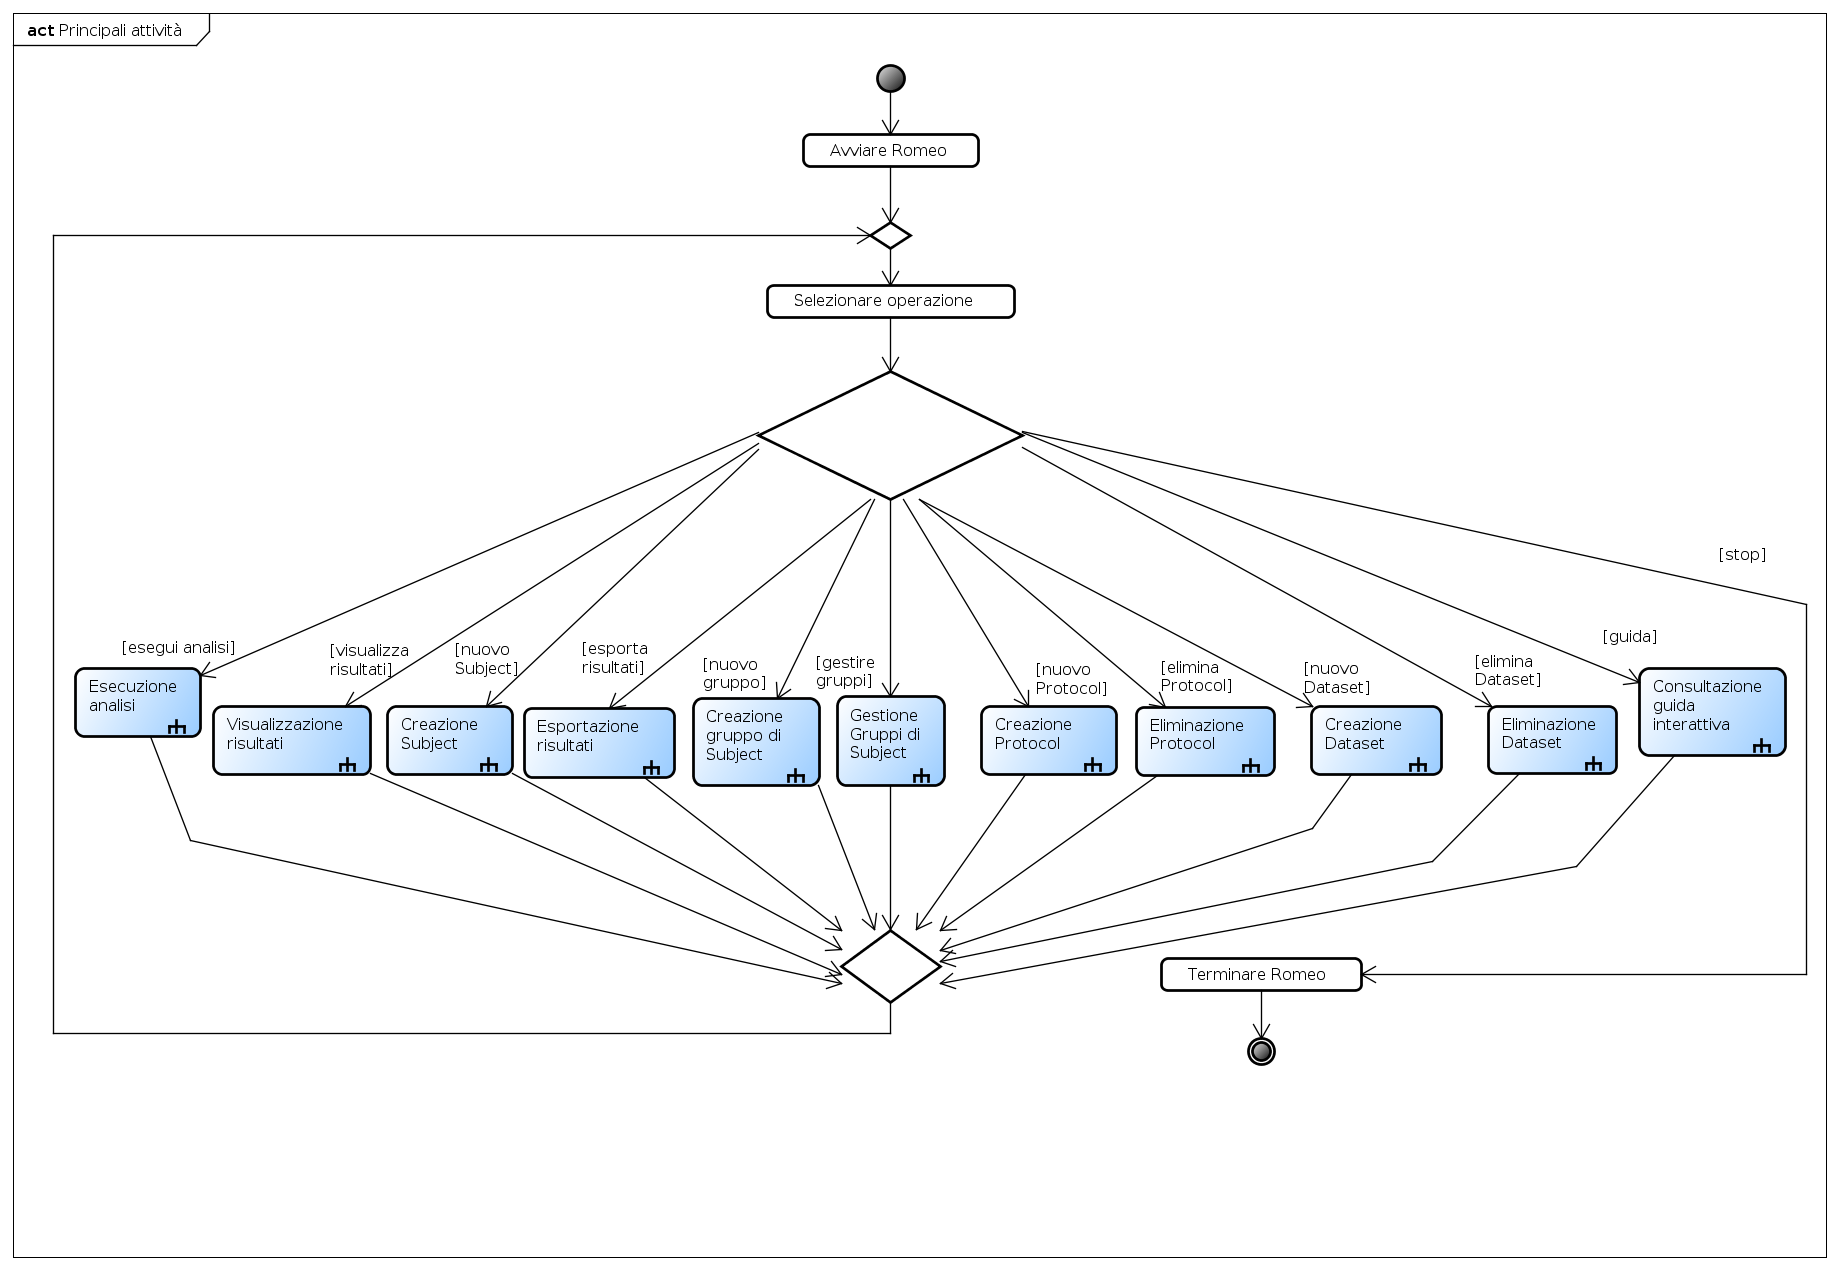
\includegraphics[scale=0.5]{./img/Diagrammi_Attivita/Principali_attivita}
	\caption{Diagramma Attività - Attività principali dell'applicativo \project{}}
	\label{generale}
\end{figure}
\end{landscape}
\pagebreak

\subsection{Creazione Subject}
\label{newSub}
\begin{figure}[!h]
	\centering
	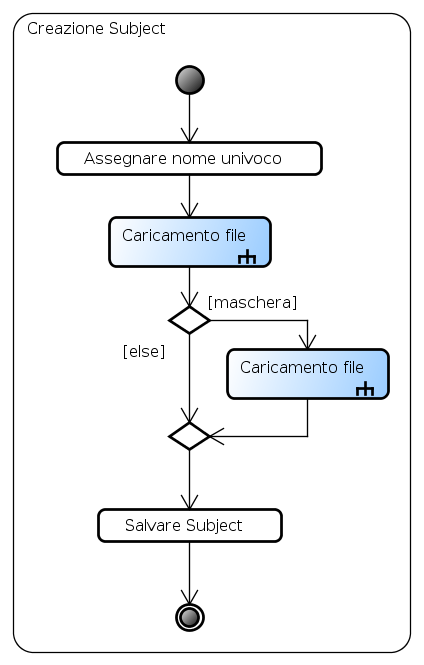
\includegraphics[scale=0.6]{./img/Diagrammi_Attivita/Creazione_Subject}
	\caption{Diagramma Attività - Creazione nuovo Subject}
	\label{newS}
\end{figure}
\paragraph{Descrizione\\}
L'attività di creazione di un nuovo Subject\glossario{} (fig. \ref{newS}), prevede innanzitutto l'assegnazione di un nome univoco al \subject{} in creazione. Successivamente è necessario caricare il file, che può essere un'immagine o un video, ed eventualmente caricare una sua maschera\glossario{}. Infine, si procede con il salvataggio del \subject{}.
\pagebreak

%caricamento di un file in romeo
\subsubsection{Caricamento file}
\label{LoadF}
\begin{figure}[!h]
	\centering
	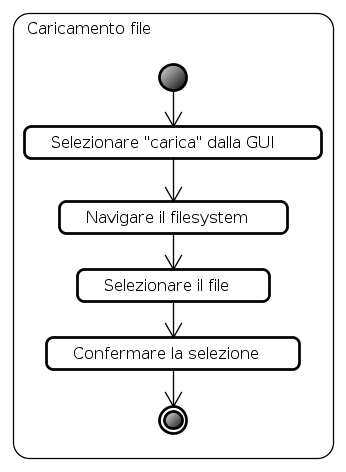
\includegraphics[scale=0.6]{./img/Diagrammi_Attivita/Caricamento_file}
	\caption{Diagramma Attività - Caricamento di un file}
	\label{Load}
\end{figure}
\paragraph{Descrizione\\}
L'attività di caricamento di un file (fig. \ref{Load}), prevede la navigazione all'interno del filesystem e la selezione del file che si desidera caricare. Infine, dopo la conferma dell'utente, si procede con l'apertura dello stesso.
\pagebreak

%creazione di un nuovo gruppo
\subsection{Creazione gruppo di Subject}
\label{newGr}
\begin{figure}[!h]
	\centering
	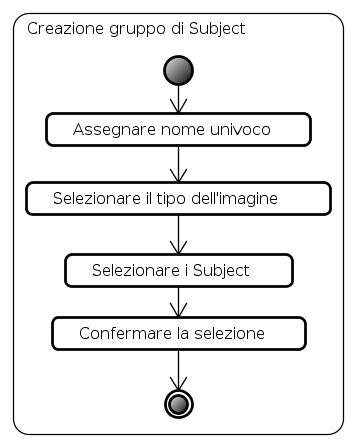
\includegraphics[scale=0.6]{./img/Diagrammi_Attivita/Creazione_gruppo_di_Subject}
	\caption{Diagramma Attività - Creazione nuovo gruppo di Subject}
	\label{newGroup}
\end{figure}
\paragraph{Descrizione\\}
L'attività di creazione di un nuovo gruppo di Subject\glossario{} (fig. \ref{newGroup}), prevede in primo luogo l'assegnazione di un nome univoco al gruppo e la scelta del tipo d'immagine (2D, 2D-t, 3D o 3D-t) che si vuole utilizzare. Successivamente è necessario selezionare i Subject\glossario{} da inserire nel gruppo, scegliendo tra quelli che hanno un'immagine associata del tipo precedentemente scelto. Infine si procede con il salvataggio del gruppo.
\pagebreak

%creazione di un nuovo protocollo
\subsection{Creazione Protocol}
\label{newPr}
\begin{figure}[!h]
	\centering
	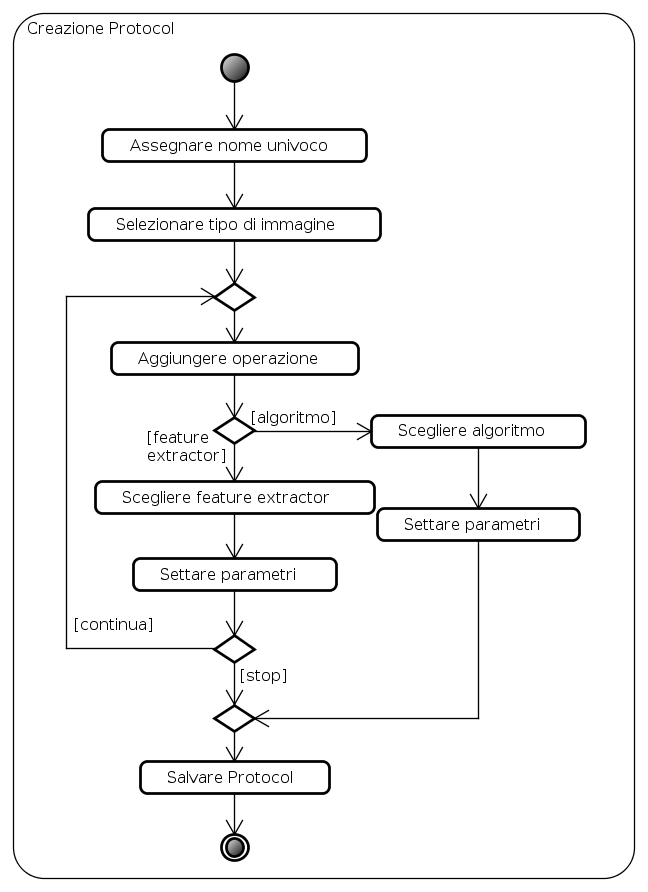
\includegraphics[scale=0.6]{./img/Diagrammi_Attivita/Creazione_Protocol}
	\caption{Diagramma Attività - Creazione di un nuovo Protocol}
	\label{newProtocol}
\end{figure}
\paragraph{Descrizione\\}
L'attività di creazione di un nuovo Protocol\glossario{} (fig. \ref{newProtocol}), prevede in primo luogo l'assegnazione di un nome univoco al Protocol\glossario{} e la scelta del tipo di immagine a cui dovrà essere applicato. \`E possibile poi selezionare le feature extractors\glossario{} che si vogliono utilizzare, dando dei valori ai parametri richiesti, e/o selezionare l'algoritmo di clustering\glossario{} dando anche per esso, dei valori ai parametri richiesti. Qualora non vengano assegnati dei valori, verranno presi quelli di default previsti dal sistema. Una volta terminata la selezione, il Protocol\glossario{} è pronto per essere salvato.
\pagebreak

%creazione di un nuovo dataset
\subsection{Creazione Dataset}
\label{newDataset}
\begin{figure}[!h]
	\centering
	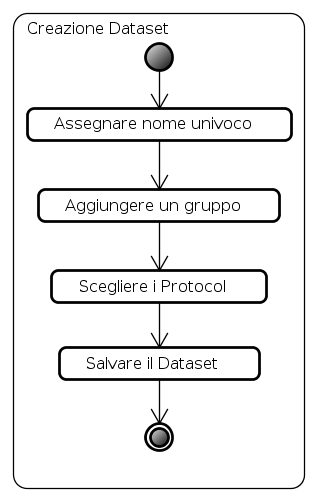
\includegraphics[scale=0.6]{./img/Diagrammi_Attivita/Creazione_Dataset}
	\caption{Diagramma Attività - Creazione di un nuovo Dataset}
	\label{newData}
\end{figure}
\paragraph{Descrizione\\}
L'attività di creazione di un nuovo Dataset\glossario{} (fig. \ref{newData}), prevede in primo luogo l'assegnazione di un nome univoco al Dataset\glossario{} in creazione e l'inserimento, in quest'ultimo, di un unico gruppo di \subject{}. Successivamente, è necessario scegliere uno o più Protocol\glossario{} da applicare al gruppo di \subject{}. I \protocol{} che potranno essere associati, saranno solo quelli compatibili in base al tipo di immagine del gruppo. Creata quest'associazione, il \dataset{} è pronto per essere salvato.
\pagebreak

%gestione gruppi di subject
\subsection{Gestione gruppi di Subject}
\label{ManageGr}
\begin{figure}[!h]
	\centering
	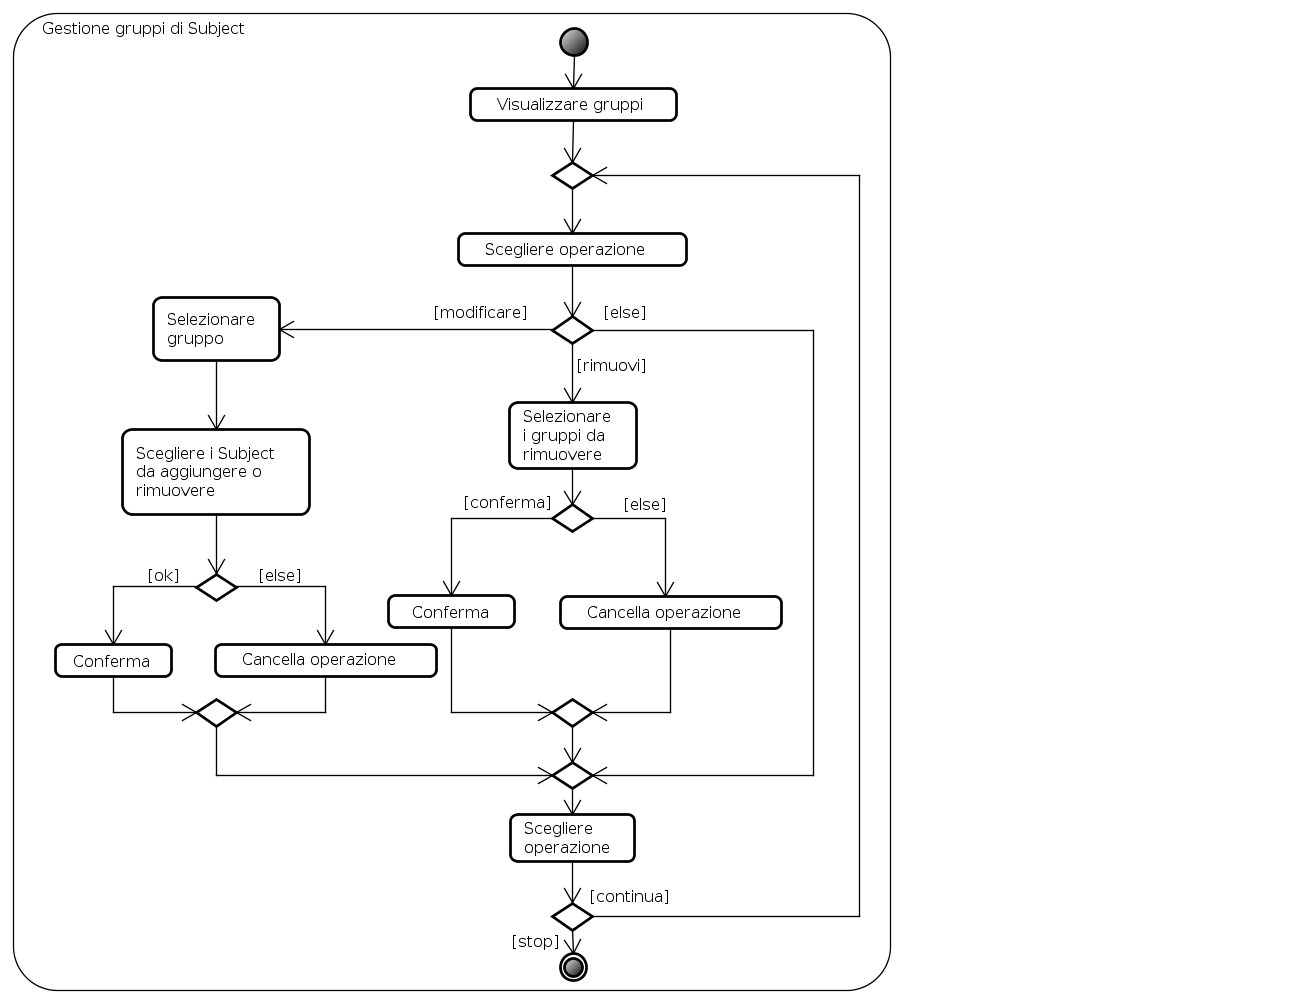
\includegraphics[scale=0.6]{./img/Diagrammi_Attivita/Gestione_gruppi_di_Subject}
	\caption{Diagramma Attività - Gestione dei gruppi di Subject}
	\label{ManageG}
\end{figure}
\paragraph{Descrizione\\}
L'attività di gestione dei gruppi di Subject\glossario{} (fig. \ref{ManageG}), dà innanzitutto la possibilità all'utente di visualizzare i gruppi salvati in quel momento nel sistema. Per ogni entità, l'utente può effettuare alcune operazioni citate di seguito.\\
\`E possibile rimuovere uno o più gruppi, visualizzarne le informazioni (Subject\glossario{} appartenenti, tipo di immagine, ecc\dots) e modificarlo. La modifica consiste nel selezionare il gruppo e scegliere quali \subject{} eliminare o inserire.\\
Per ogni singola operazione, è necessaria la conferma da parte dell'utente, che può inoltre annullarla in qualsiasi momento.
\pagebreak

%gestione dei protocolli
\subsection{Eliminazione Protocol}
\label{ManageProt}
\begin{figure}[!h]
	\centering
	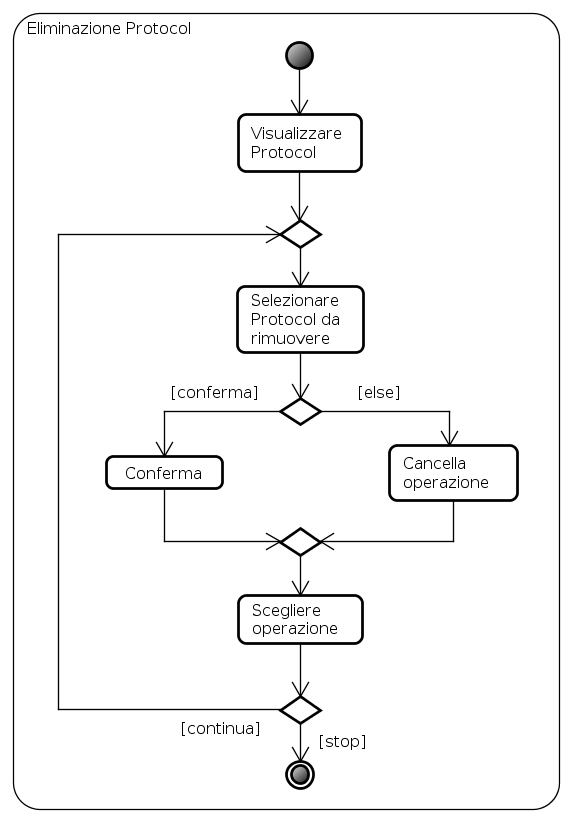
\includegraphics[scale=0.6]{./img/Diagrammi_Attivita/Eliminazione_Protocol}
	\caption{Diagramma Attività - Eliminazione dei Protocol}
	\label{ManagePr}
\end{figure}
\paragraph{Descrizione\\}
L'attività di eliminazione dei Protocol\glossario{} (fig. \ref{ManagePr}), dà la possibilità all'utente di eliminare uno o più Protocol\glossario{} presenti in quel momento nel sistema. La cancellazione consiste nel selezionare i \protocol{} che si vogliono eliminare e successivamente confermare la cancellazione. In qualsiasi momento, l'utente può decidere di abbandonare l'operazione e di ritornare al menù principale.
\pagebreak

%gestione dei dataset
\subsection{Eliminazione Dataset}
\label{ManageDataset}
\begin{figure}[!h]
	\centering
	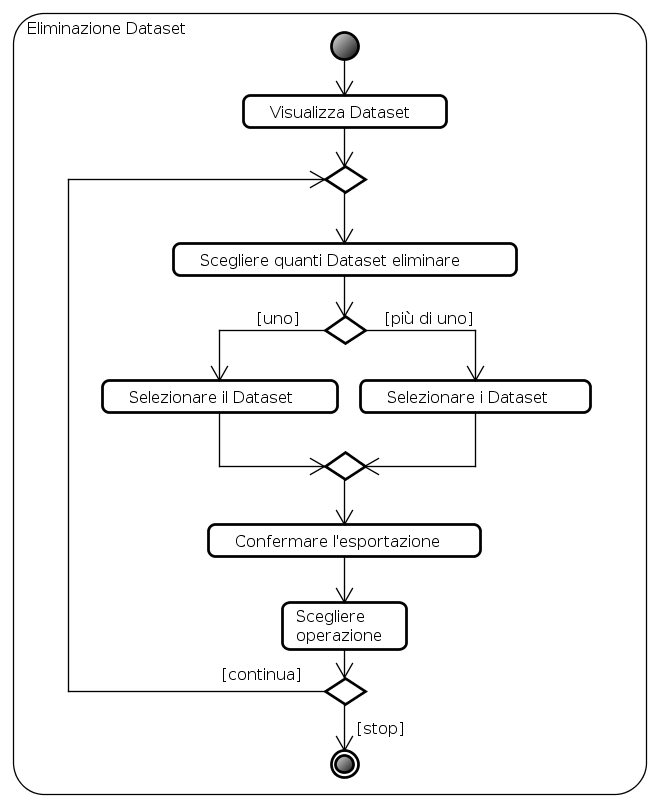
\includegraphics[scale=0.6]{./img/Diagrammi_Attivita/Eliminazione_Dataset}
	\caption{Diagramma Attività - Eliminazione dei Dataset}
	\label{ManageData}
\end{figure}
\paragraph{Descrizione\\}
L'attività di eliminazione dei \dataset{} (fig. \ref{ManageData}), dà la possibilità all'utente di eliminare uno o più \dataset{} presenti in quel momento nel sistema. La cancellazione consiste nel selezionare i \dataset{} che si vogliono eliminare e successivamente confermare la cancellazione. In qualsiasi momento, l'utente può decidere di abbandonare l'operazione e di ritornare al menù principale.
\pagebreak

\subsection{Esecuzione analisi}
\label{diagramma_analisi}
\begin{figure}[!h]
\begin{center}
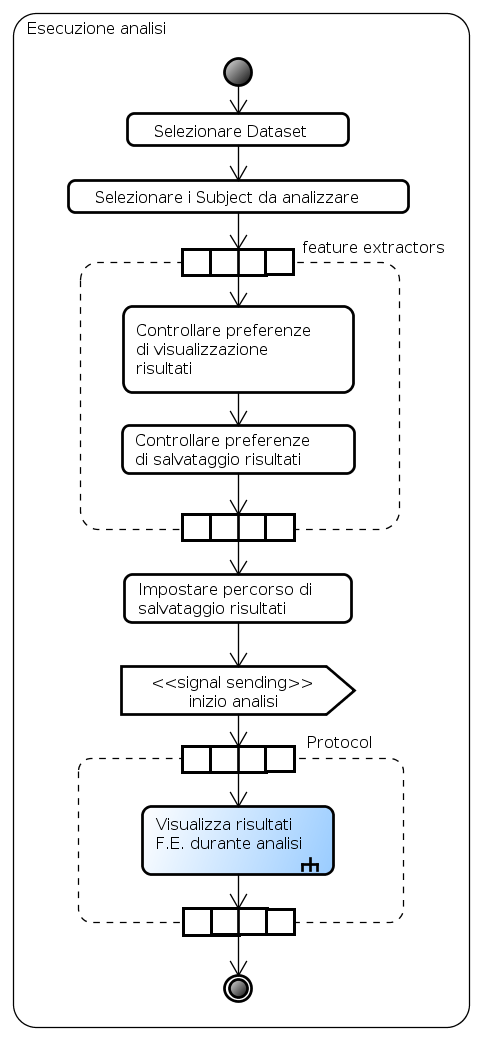
\includegraphics[scale=0.6]{./img/Diagrammi_Attivita/Esecuzione_analisi}
\caption{Diagramma attività - Esecuzione analisi}
\end{center}
\end{figure}
\paragraph{Descrizione\\}
Il diagramma mostra come l'utente interagisce con il sistema durante l'analisi. 
\\In primo luogo, l'utente deve selezionare il \dataset{} su cui vuole eseguire l'analisi. Successivamente, può scegliere su quali \subject{} appartenenti al gruppo del \dataset{}, applicare i \protocol{}. Nel caso in cui l'utente non selezioni alcun \subject{}, l'analisi verrà effettuata su tutto il gruppo di \subject{}. In seguito, è possibile selezionare di quali feature extractor\glossario{} si vogliono visualizzare i risultati, durante l'analisi. Questa opzione darà la possibilità all'utente di decidere se le feature extractor\glossario{} applicate al \subject{}, sono efficaci. In caso contrario, sarà possibile interrompere l'esecuzione dell'analisi senza dover aspettare il completamento dell'intera analisi.
\\L'ultima operazione prima di avviare l'analisi, consiste nell'indicare la directory in cui si vogliono salvare i risultati.

\subsubsection{Visualizzazione dei risultati delle feature extractor durante l'analisi}
\label{risultati_fe_durante_analisi}
\begin{figure}[!h]
\begin{center}
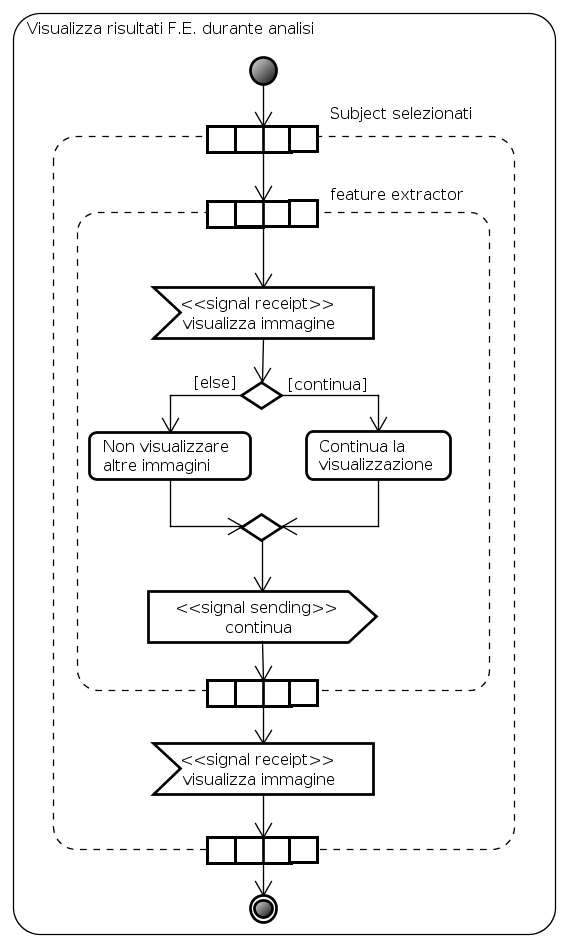
\includegraphics[scale=0.6]{./img/Diagrammi_Attivita/Visualizza_risultati_durante_analisi}
\caption{Diagramma attività - Visualizzazione risultati delle feature extractor durante l'analisi}
\end{center}
\end{figure}
\paragraph{Descrizione\\}
Il diagramma mostra l'interazione tra utente e sistema, nel momento in cui quest'ultimo sta applicando le feature extractor\glossario{} ad un \subject{}. Per ogni risultato estratto dal \subject{}, l'utente è chiamato a dare la sua conferma per la prosecuzione dell'analisi. In alternativa, può decidere di saltare in blocco la visualizzazione dei successivi risultati o di annullare completamente l'analisi.
\pagebreak

\subsection{Visualizzazione risultati}
\label{seeAnalysis}
\begin{figure}[!h]
	\centering
	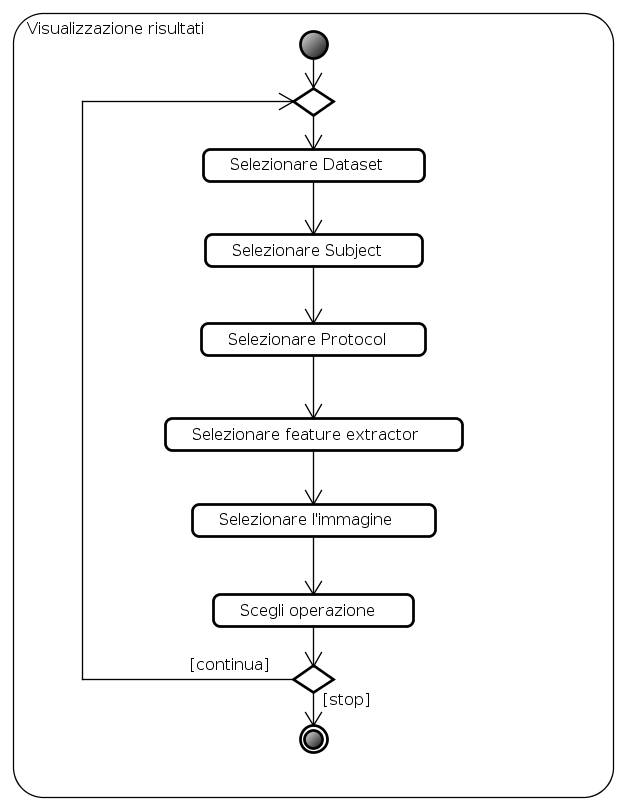
\includegraphics[scale=0.6]{./img/Diagrammi_Attivita/Visualizzazione_risultati}
	\caption{Diagramma Attività - Visualizzazione dei risultati delle analisi}
	\label{showAnalysis}
\end{figure}
\paragraph{Descrizione\\}
Quest'attività permette all'utente di visualizzare i risultati delle analisi precedentemente effettuate.
\\Il sistema fornirà l'elenco dei \dataset{} su cui è stata avviata un analisi e l'utente dovrà selezionare quello di suo interesse. Successivamente, l'utente dovrà selezionare il \subject{} di cui vuole visualizzare i risultati. Infine, sarà possibile navigare tra i vari \protocol{} in maniera da poter scegliere quali immagini (estratte da feature extractors\glossario{} o algoritmi di clustering) visualizzare. 
\pagebreak

\subsection{Esportazione risultati}
\label{seeAnalysis}
\begin{figure}[!h]
	\centering
	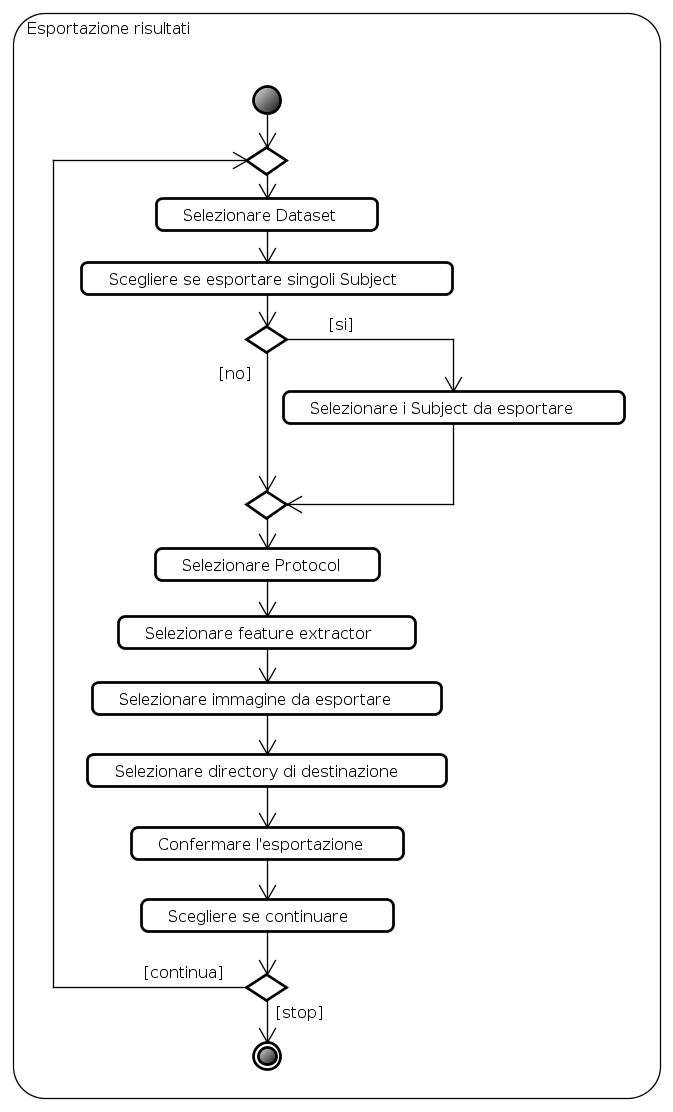
\includegraphics[scale=0.6]{./img/Diagrammi_Attivita/Esportazione_risultati}
	\caption{Diagramma Attività - Esportazione dei risultati delle analisi}
	\label{espAnalysis}
\end{figure}
\paragraph{Descrizione\\}
Quest'attività permette all'utente di esportare i risultati delle analisi precedentemente effettuate.
\\Il sistema fornirà l'elenco dei \dataset{} su cui è stata avviata un analisi e l'utente dovrà selezionare quello di suo interesse. Successivamente, l'utente dovrà selezionare il \subject{} di cui vuole esportare i risultati. Infine, sarà possibile navigare tra i vari \protocol{} in maniera da poter scegliere quali immagini (estratte da feature extractors\glossario{} o algoritmi di clustering) esportare. 
\pagebreak

%apertura della guida
\subsection{Consultazione guida interattiva}
\label{guide}
\begin{figure}[!h]
	\centering
	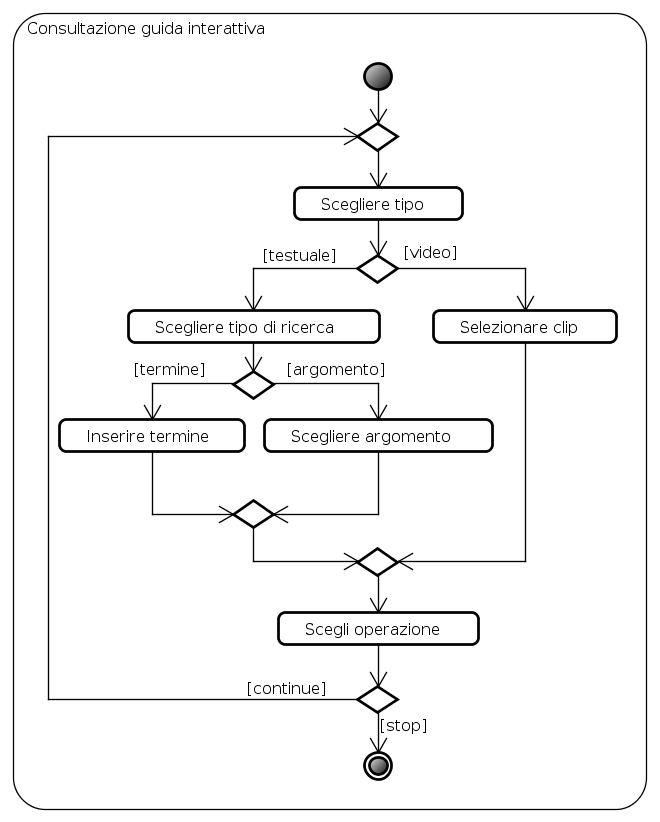
\includegraphics[scale=0.6]{./img/Diagrammi_Attivita/Consultazione_guida_interattiva}
	\caption{Diagramma Attività - Consultazione della guida interattiva}
	\label{openG}
\end{figure}
\paragraph{Descrizione\\}
L'attività di consultazione della guida (fig. \ref{openG}), fornisce all'utente la possibilità di essere guidato nell'utilizzo del software \project{}. L'utente può scegliere se aprire la guida testuale oppure la guida video. Per quanto riguarda la guida testuale, ha a disposizione la ricerca per argomento oppure per termine, mentre per quanto riguarda la guida video, potrà scegliere il clip di interesse. Una volta terminata la ricerca, può continuare con una nuova ricerca oppure chiuderla.